\section{Concept}
\label{sec:concept}

In this paper, we adovocate a concept of mobility CPS in the cloud.
Many mobility CPS applications are battery-operated.
They cannot accommodate large power consumers unless they equip special
battery facilities.
Integrating cloud technology allows computations and data to be
offloaded over the network and we are freed from power consumption
issues.
For simplicity of description, we present our concept in the context of
autonomous driving, but it is highly applicable for other mobility CPS
applications.

\subsection{Big Data}

Grand challenges of mobility CPS include the modeling of the physical
world that underlies the real-time understanding of the physical world
including enviromental perception and motion control.
The modeling of the physical world requires accumulative collection of
real-world data.
This is often referred to as ``Big Data'' on the recent trend.

\begin{figure}[!t]
 \centering
 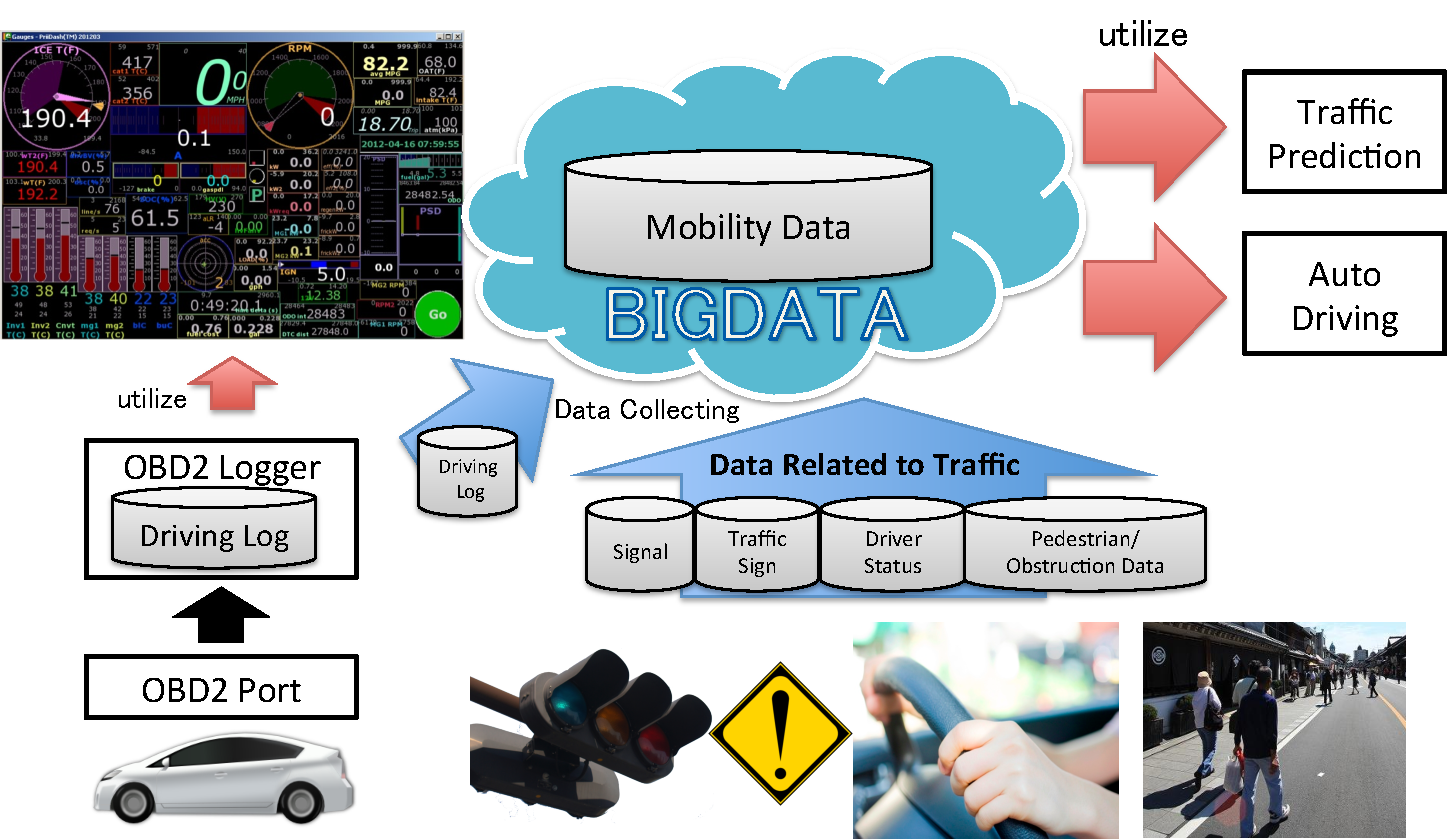
\includegraphics[width=\hsize]{fig/OBD2.pdf}
 \caption{Collecting automotive data.}
 \label{fig:obd2}
\end{figure}

Fig. \ref{fig:obd2} illustrates an example of collecting automotive data
through the on-board diagnosis (OBD) connectors as well as environmental
and human data.
We are building this system using commodity products. 
The automotive data can be obtained as CAN bus data while the
environmental and human data can be captured using mobile devices such
as smartphones.
While the data volume is a challenging issue and especially a
cummulative collection of laser sensor data and camera images produces a
significant amont of data, this is more or less a typical information
and communication technology (ICT) problem but not necessarily
associated with CPS and latency matters.
Currently we store the collected data in a vehicular computer and move
them to database systems and storage servers offline.
Although this approach is sufficient to collect mobility data, it means
that CPS applications need to communicate with these Big Data systems at
runtime to adapt to the dynamically changing physical-world environment.
We will discuss these issues in Section \ref{sec:perception} and
\ref{sec:control}.

\subsection{Perception}
\label{sec:perception}

\begin{figure}[!t]
 \centering
 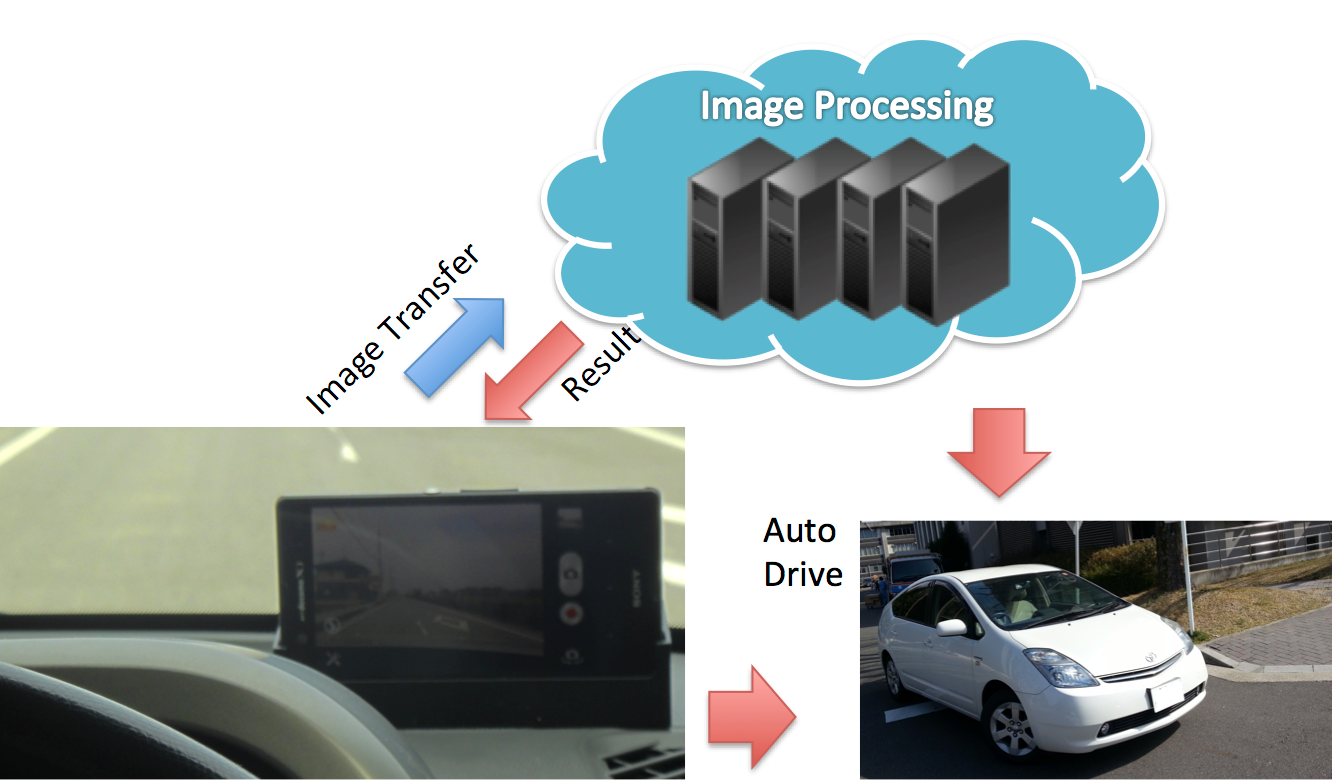
\includegraphics[width=\hsize]{fig/TIPIC.pdf}
 \caption{Networked image processing.}
 \label{fig:tipic}
\end{figure}

The computional cost of real-time perception in mobility CPS is highly
expensive.
The perception algorithm is often computationally complex and the volume
of input data from laser sensors and cameras is not afforable for mobile
embedded systems.

\subsection{Control}
\label{sec:control}

\begin{figure}[!t]
 \centering
 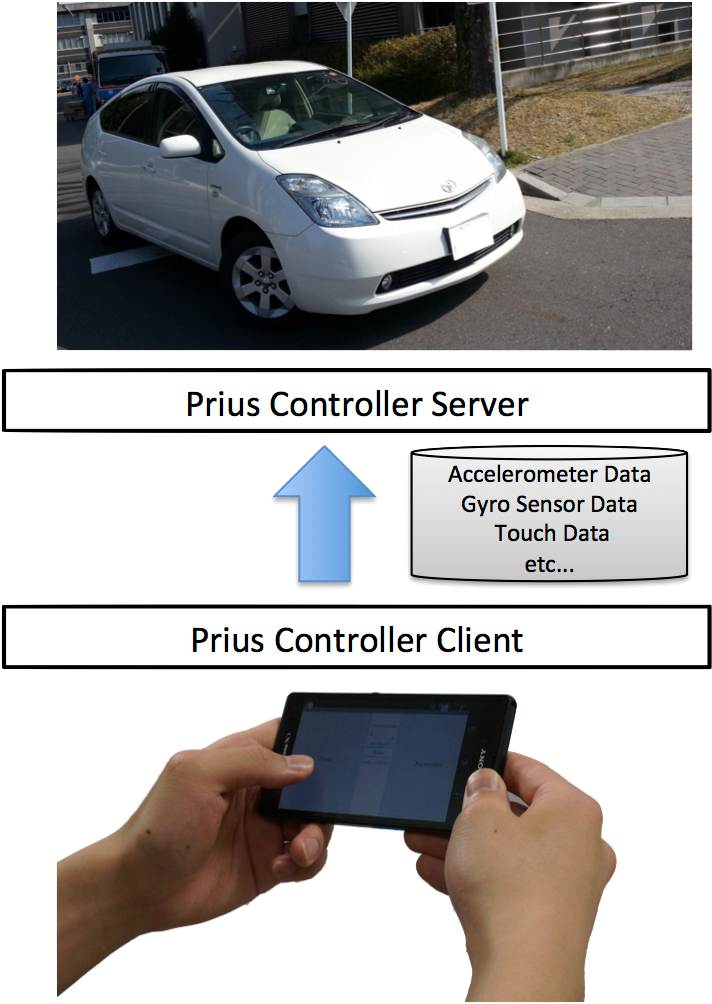
\includegraphics[width=0.75\hsize]{fig/Andrive.pdf}
 \caption{A smartphone application for remote vehicle control.}
 \label{fig:andrive}
\end{figure}

